%http://cs.pugetsound.edu/~jross/courses/cs240/project/requirements/
%Animation Group
\documentclass[12pt]{article}
\usepackage{graphicx}
\begin{document}

% Front Page
\begin{titlepage}
	\begin{center}
	\huge  Edith \\
	\vspace*{\fill}%
 	\huge \textsc{\textbf{Animation System \\Intermediate Report} }	
	\bigskip 
	\rule{130mm}{.1pt}
	\textsc{\textbf{October 7, 2013 \\ Revised: October 17, 2013} \\ }	
	\vspace*{\fill}%
	Eric Lund \\
	Kramer Canfield \\ 
	Zeke Rosenberg \\
	Calder Whiteley \\
	Jon Youmans
	\end{center}
\end{titlepage}

\section{\emph{Animation System Structure}}%Create a section for the introduction
\begin{enumerate}
\item Parser
\begin{enumerate}
\item The Animation System will be receiving instructions for animations in JSON format. This subsystem will take the instructions and actually call the functions with correct inputs. Our required interface is JSON, but more specifically a JSON entry with the following elements:
\item \{"function name" : "jump(x1, x2, y1, y2)", "Image Name": "example.png", "sound name": "soundFile.mp3"\}
\item There will be some instructions that might not have some of these fields; 'null' will be acceptable.
\end{enumerate}

\item Controller
\begin{enumerate}
\item Once we have parsed JSON inputs into instructions, the next subsystem will carry out those instructions and make calls to the HTML5 canvas. This subsystem will have several important interactions with other pieces.
\item This system will take the raw data about instructions- with files waiting to be loaded until the canvas is ready to actually animate. For example, this system takes the instruction to move to the right, and 'remembers' the last position of an object, and the new position with x=x+5 (example). This information will be stored in a 'frame' array so that fastforward/rewind will allow the user to 'step' through the program if they desire.
\item This system will also take the instructions and call them on the canvas. Therefore, this is where the majority of functions that will be written, and can be called if given the correct input.
\end{enumerate}

\item Scene Array
\begin{enumerate}
\item The Scene Array sub-component simply holds a list of frames, each frame being one step of the animation process. These will be stored in an array so that playback control functions (called by another team) will allow the user to select a time to view from, and the Scene Array can then get the necessary media and display it. 
\end{enumerate}

\item Interactions
\begin{enumerate}
\item The animation system will have no direct interaction with the ``programmer"; it is a part of the abstraction process we are doing on the animation to make it easier to do simple animations. Therefore, we have no mock-up of our end product, as it is reliant on the canvas created for us as well as buttons and other UI aspects we are not dealing with.
\item The Animation System interacts with the Story Creator module, who feeds us the JSON instructions to be parsed and carried out. It also interacts with the visual editor team, which will be providing the images, sounds, etc. to be used following the JSON instructions. Finally, we will be giving our output to the (some other team here) to be painted on the canvas.
\item The only other requirement for the Animation system is that we are using a 3rd party library, 'OCanvas', to make animations easier (and cooler!). This library works directly with an HTML5 canvas, so there are minimal if any changes from other teams. This can be found at http://ocanvas.org/docs

\end{enumerate}



\end{enumerate}

\subsection{Activity Diagram}
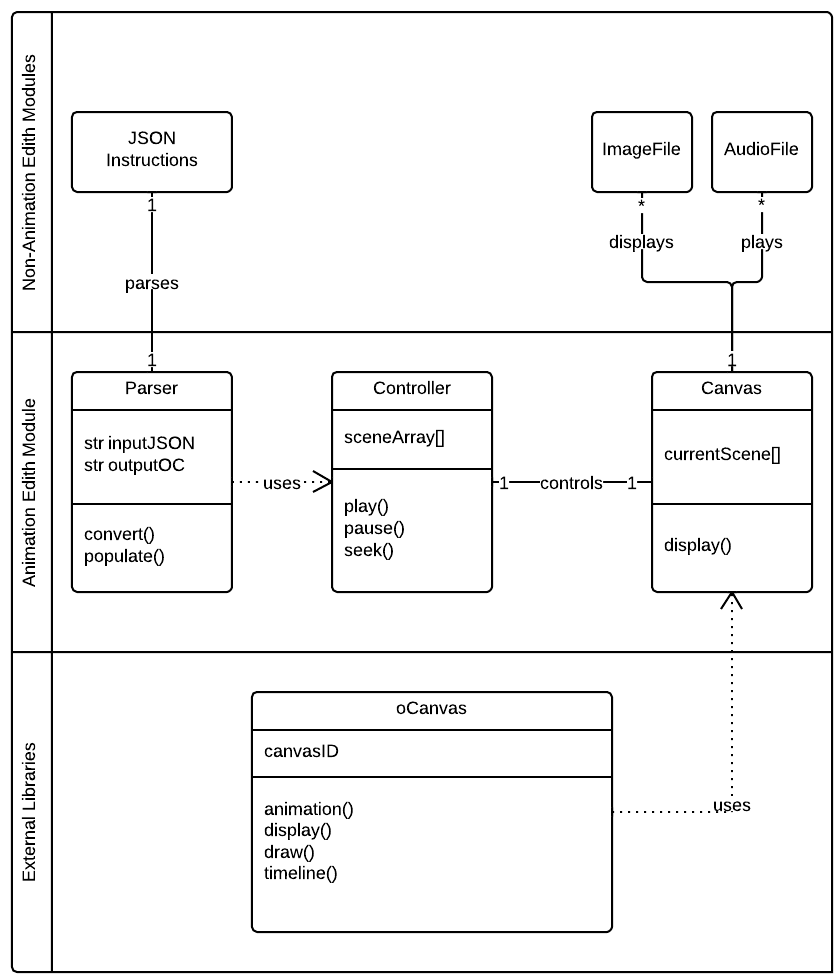
\includegraphics[scale=.45]{AnimationUMLClassDiagram.png}
\\UML Class Diagram
\pagebreak

%Glossary/References
\section{\emph{Glossary/References}}
Glossary:
\begin{itemize}
	\item Programmer: The individual who is using Edith through his/her web browser to learn how to program.
	\item Sprite: a computer graphic that may be moved on-screen and otherwise manipulated as a single entity (New Oxford American Dictionary (American English))
\end{itemize}
	

	
\end{document}
